% The framework figure of the paper: PACE's symbolic pipeline and the digital twin that validates it.
%   cd experiments && latexmk -pdf framework_figure.tex && cp framework_figure.pdf ../build/figures/framework.pdf
% Built at the LNCS text width (122 mm) so that every font size is the printed size.
\documentclass[tikz,border=0pt]{standalone}
\usepackage[T1]{fontenc}
\usepackage[scaled=0.92]{helvet}
\usepackage[varvw]{newtxmath}
\renewcommand{\familydefault}{\sfdefault}
\usetikzlibrary{arrows.meta,calc}
\hyphenpenalty=10000
\exhyphenpenalty=10000

% effort colors of the twin figure (experiments/make_twin_figures.py)
\definecolor{low}{HTML}{2CA02C}
\definecolor{medium}{HTML}{E6A100}
\definecolor{high}{HTML}{D62728}
\definecolor{pace}{HTML}{1F5FA8}
\definecolor{pacebg}{HTML}{EDF2F9}
\definecolor{twin}{HTML}{2A7F62}
\definecolor{twinbg}{HTML}{EAF4EF}
\definecolor{ink}{HTML}{222428}
\definecolor{soft}{HTML}{50555C}

\newcommand{\body}{\fontsize{6.3}{7.4}\selectfont\color{soft}}
\newcommand{\head}{\fontsize{7.1}{7.4}\selectfont\bfseries\color{ink}}
\newcommand{\lane}{\fontsize{5.8}{6.5}\selectfont\bfseries}

\tikzset{
  box/.style={draw=#1, line width=0.6pt, rounded corners=2pt, fill=white, align=center,
              inner xsep=2pt, inner ysep=0pt, anchor=south west, font=\body},
  flow/.style={-{Stealth[length=4.2pt,width=3.4pt]}, line width=0.75pt, draw=ink},
  pill/.style={rounded corners=2.2pt, fill=#1, text=white, inner xsep=3pt, inner ysep=1.5pt,
               font=\fontsize{6.1}{6.6}\selectfont\bfseries, minimum width=20mm, align=center},
  note/.style={inner sep=1.5pt, font=\fontsize{6.1}{7}\selectfont\color{soft}},
}

% a box from (x0,y0) to (x1,y1), in centimeters: name, color, x0, y0, x1, y1, title, text
\newcommand{\cell}[8]{%
  \node[box=#2, minimum width=#5cm-#3cm, minimum height=#6cm-#4cm, text width=#5cm-#3cm-4pt]
    (#1) at (#3,#4) {{\head #7}\\[2.5pt]#8};}

\begin{document}
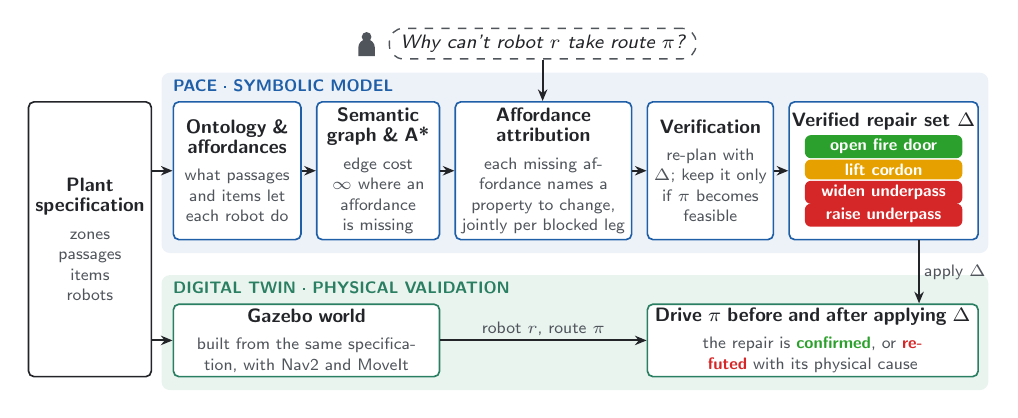
\begin{tikzpicture}[x=1cm,y=1cm]
  % lanes
  \fill[pacebg, rounded corners=3pt] (1.70,1.74) rectangle (12.2,4.03);
  \fill[twinbg, rounded corners=3pt] (1.70,0.00) rectangle (12.2,1.46);
  \node[anchor=north west, text=pace, inner sep=0] at (1.84,3.95) {\lane PACE\,\,\textperiodcentered\,\,SYMBOLIC MODEL};
  \node[anchor=north west, text=twin, inner sep=0] at (1.84,1.38) {\lane DIGITAL TWIN\,\,\textperiodcentered\,\,PHYSICAL VALIDATION};

  % the shared input
  \cell{spec}{ink}{0.00}{0.16}{1.56}{3.65}{Plant\\specification}{zones\\passages\\items\\robots}

  % the symbolic pipeline
  \cell{onto}{pace}{1.84}{1.90}{3.46}{3.65}{Ontology \&\\affordances}{what passages and items let each robot do}
  \cell{graph}{pace}{3.66}{1.90}{5.22}{3.65}{Semantic\\graph \& A*}{edge cost $\infty$ where an affordance is missing}
  \cell{attr}{pace}{5.42}{1.90}{7.66}{3.65}{Affordance\\attribution}{each missing affordance names a property to change, jointly per blocked leg}
  \cell{verify}{pace}{7.86}{1.90}{9.46}{3.65}{Verification}{re-plan with $\Delta$; keep it only if $\pi$ becomes feasible}
  \node[box=pace, minimum width=2.40cm, minimum height=1.75cm] (set) at (9.66,1.90) {};
  \node[anchor=north, inner sep=0] at ($(set.north)+(0,-0.14)$) {\head Verified repair set $\Delta$};
  \node[pill=low]    at ($(set.north)+(0,-0.58)$) {open fire door};
  \node[pill=medium] at ($(set.north)+(0,-0.87)$) {lift cordon};
  \node[pill=high]   at ($(set.north)+(0,-1.16)$) {widen underpass};
  \node[pill=high]   at ($(set.north)+(0,-1.45)$) {raise underpass};

  % the twin
  \cell{world}{twin}{1.84}{0.16}{5.22}{1.08}{Gazebo world}{built from the same specification, with Nav2 and MoveIt}
  \cell{drive}{twin}{7.86}{0.16}{12.06}{1.08}{Drive $\pi$ before and after applying $\Delta$}%
    {the repair is \textcolor{low}{\bfseries confirmed}, or \textcolor{high}{\bfseries refuted} with its physical cause}

  % the query
  \node[draw=soft, dashed, line width=0.5pt, rounded corners=5pt, fill=white, inner xsep=4pt, inner ysep=2.4pt,
        font=\fontsize{6.6}{7.4}\selectfont\itshape\color{ink}] (q) at (6.54,4.40)
        {Why can't robot $r$ take route $\pi$?};
  \begin{scope}[shift={($(q.west)+(-0.28,-0.03)$)}]
    \fill[soft] (0,0.115) circle (0.062);
    \fill[soft] (-0.105,-0.13) -- (-0.105,-0.02) arc (180:0:0.105) -- (0.105,-0.13) -- cycle;
  \end{scope}

  % flows
  \draw[flow] (spec.east |- onto.west) -- (onto.west);
  \draw[flow] (spec.east |- world.west) -- (world.west);
  \draw[flow] (onto) -- (graph);
  \draw[flow] (graph) -- (attr);
  \draw[flow] (attr) -- (verify);
  \draw[flow] (verify) -- (set);
  \draw[flow] (q.south) -- (q.south |- attr.north);
  \draw[flow] (world) -- node[note, above] {robot $r$, route $\pi$} (drive);
  \coordinate (d0) at ($(set.south)+(0.45,0)$);
  \draw[flow] (d0) -- node[note, right] {apply $\Delta$} (d0 |- drive.north);
\end{tikzpicture}
\end{document}
